\documentclass[tikz,border=8pt]{standalone}
\usepackage{amsmath}
\begin{document}
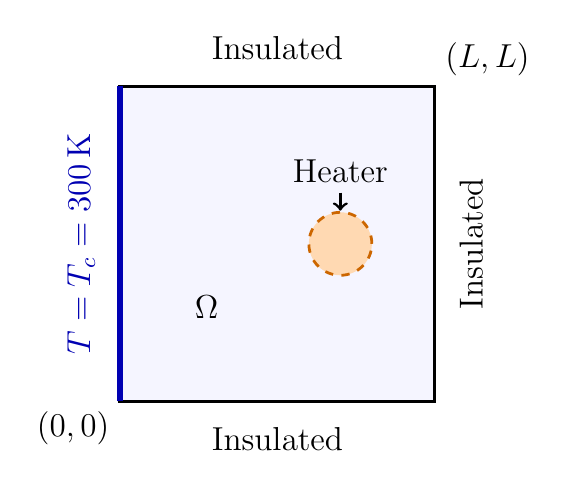
\begin{tikzpicture}[font=\large,line width=1pt]
\fill[blue!4] (0,0) rectangle (4,4);
\draw (0,0) rectangle (4,4);
\draw[blue!70!black,line width=2pt] (0,0)--(0,4);
\node[rotate=90,above,text=blue!70!black] at (-0.18,2) {$T=T_c=300\,\mathrm K$};
\node[rotate=90,below] at (4.18,2) {Insulated};
\node[above] at (2,4.2) {Insulated};
\node[below] at (2,-0.2) {Insulated};
\fill[orange!30] (2.8,2) circle (0.4);
\draw[orange!80!black,dashed] (2.8,2) circle (0.4);
\node[above] at (2.8,2.65) {Heater};
\draw[->] (2.8,2.65)--(2.8,2.42);
\node at (1.1,1.2) {$\Omega$};
\node[below left] at (0,0) {$(0,0)$};
\node[above right] at (4,4) {$(L,L)$};
\end{tikzpicture}
\end{document}
